\section{PCB Design}\label{sec:PCB}
\todo[color=c05c,inline]{testing the colors}

To be able to test the proposed topology,
a Printed Circuit Board (PCB) had to be made.
We got some guidance in this process by Sagar Mahajal,\todo[color=c05c]{reference him?}.
a Ph.D. student working on the same project.

Because this circuit is designed for power electronics,
some different precautions had to be made from conventional PCB design.
The copper traces had to be wide enough to accommodate the currents going through
and spaced apart enough to prevent the potential difference from creating sparks between them.

\subsection{Two Stage PCB}
To get familiar with designing power electronics PCBs,
we started out designing a two stage version of the proposed topology.
Because we already had some familiarities with EAGLE from previous projects,
we used EAGLE for the first design attempts.

\begin{figure}[H]
	\begin{center}
	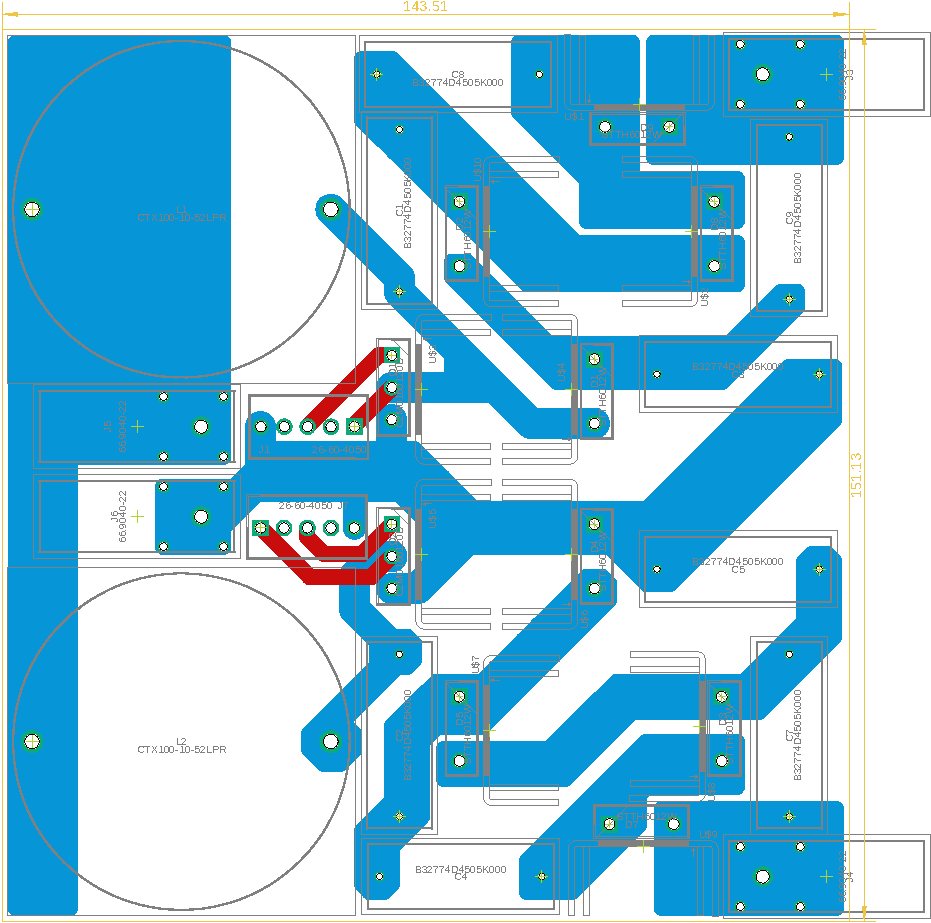
\includegraphics[width=0.6\textwidth]{figures/05cPCBdesign/2NX_interleaved_boost_converter_EAGLE_BY_DANIEL.pdf}
	\end{center}
	\caption{PCB Layout for a two stage 2NX Interleaved Boost Converter}
	\label{fig:2nxeagle}
\end{figure}

The most noticeable differences between logic PCBs and power PCBs for us were
the increased trace width and the size of the individual components.

The finished design can be seen in Figure \ref{fig:2nxeagle}.
The red traces are logical signals,
located on the top layer of the PCB,
blue are power traces located on the bottom layer.
The power traces can be observed to be broader than the logic,
and were drawn as polygons,
to use the biggest available surface area.
The logical signals are designed to be as short as possible
and to be located as far from the power traces as possible,
to minimize interference.

Precautions were made in respect to the method of manufacturing,
because acute angles between two legs of a trace can lead to cracks in the trace when etching.
To prevent this from happening,
more copper was added in the areas in question to create obtuse angles.
A detailed view of this can be seen in Figure \ref{fig:2nxeagledetail}.
\begin{figure}[H]
	\begin{center}
	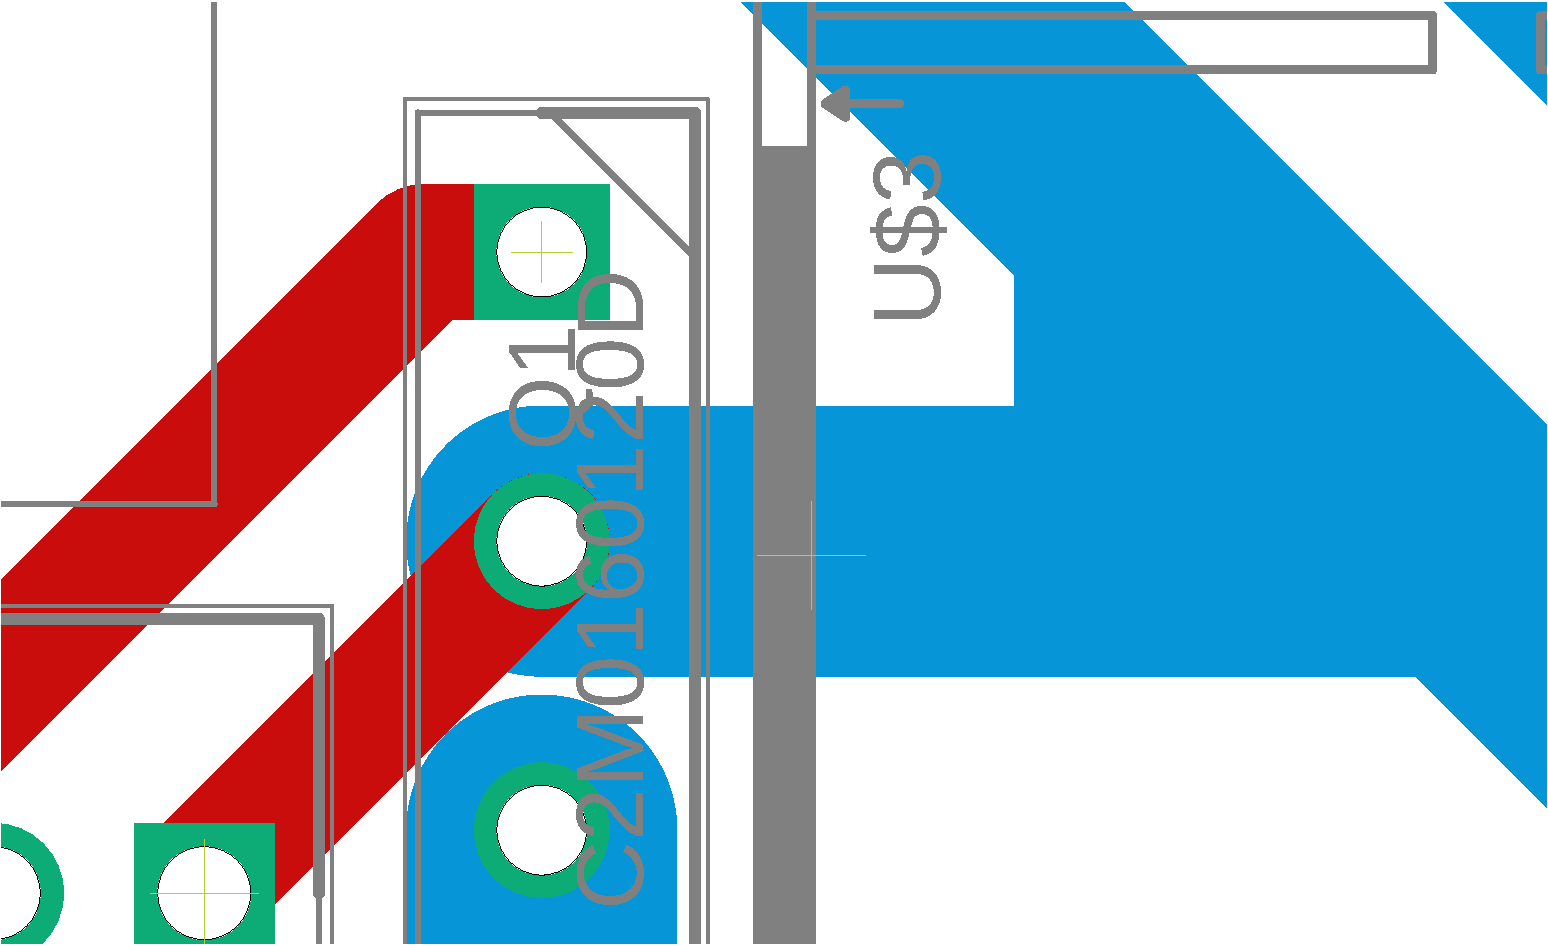
\includegraphics[width=0.6\textwidth]{figures/05cPCBdesign/2NX_interleaved_boost_converter_EAGLE_BY_DANIEL_DETAIL.pdf}
	\end{center}
	\caption{Detailed view of PCB Layout}
	\label{fig:2nxeagledetail}
\end{figure}

\subsection{Three Stage PCB}\label{sub:3sPCB}
To lessen our workload our supervisor put us into contact with Sagar Mahajan \todo[color=c05c]{cite to his linkedin?}
Because there already existed layouts for a three stage version of the proposed topology,
which were given to us by our supervisor,
we decided to continue working based on the already existing files.
\todo[color=c05c,inline]{something about diptrace, and collaboration with Sagar}